\documentclass[t]{beamer}
\usepackage[utf8]{inputenc}
\usepackage{amsmath,amsfonts,amsthm,amstext,amssymb, xcolor, tikz, pgf, polynom}

% ----------------------------------------------------------
% Theme Setup

% Use Metropolis Theme
\usetheme[numbering=fraction]{metropolis}
\setbeamertemplate{blocks}[rounded][shadow=false]
\makeatletter
\setlength{\metropolis@titleseparator@linewidth}{1pt}
\makeatother

% Define Colors
\definecolor{chargerblue}{HTML}{002764}
\definecolor{chargerred}{HTML}{e02034}
\definecolor{bggray}{HTML}{d0d3d4}

% Set Colors
\setbeamercolor{title}{fg=chargerblue}
\setbeamercolor{background canvas}{bg=white}
\setbeamercolor{title separator}{fg=chargerred}
\setbeamercolor{structure}{fg=chargerblue}
\setbeamercolor{frametitle}{fg=white, bg=chargerblue}
\setbeamercolor*{normal text}{fg=chargerblue}
\setbeamercolor*{block body}{bg=bggray}
\setbeamercolor*{block title}{bg=chargerblue, fg=white}
% ----------------------------------------------------------

% ----------------------------------------------------------
% Custom Definitions, Commands, Environments, etc.

% Sets of numbers
\def\R{\mathbb{R}} % The reals
\def\N{\mathbb{N}} % The naturals
\def\Z{\mathbb{Z}} % The integers
\def\Q{\mathbb{Q}} % The rationals

% Blank space
\newcommand{\blank}[1]{\underline{\hspace{#1}}} % Blank space

% Fitted inclusion symbols
\newcommand{\fp}[1]{\left({#1}\right)} % Fitted parentheses around content
\newcommand{\fb}[1]{\left[{#1}\right]} % Fitted brackets
\newcommand{\set}[1]{\left\{{#1}\right\}} % Fitted braces (useful for sets)
\newcommand{\av}[1]{\left|{#1}\right|} % Fitted absolute value bars



% Coordinate Plane (Four-Quadrant)
\def\coordplane {
	\begin{tikzpicture}		\draw[step=0.25cm,black,very thin,opacity=0.25] (-2.5cm, -2.5cm) grid (2.5cm, 2.5cm);
	\draw[<->,thick,black] (-2.5cm, 0) -- (2.5cm, 0) node[anchor=north west,pos=0.94,font=\scriptsize]{$x$};
	\draw[<->,thick,black] (0,-2.5cm) -- (0, 2.5cm) node[anchor=south east,font=\scriptsize,pos=0.94]{$y$};
	\end{tikzpicture}
}

% Coordinate Plane (One-Quadrant)
\def\onequad {
	\begin{tikzpicture}
	\draw[step=0.25cm, black, very thin, opacity=0.25] (0,0) grid (7.5cm,5cm);
	\draw[->, thick, black] (0,0) -- (7.5cm, 0) node[anchor=north west,font=\scriptsize,pos=0.94]{$x$};
	\draw[->, black, thick] (0,0) -- (0,5cm) node[anchor=south east,font=\scriptsize,pos=0.94]{$y$};
	\end{tikzpicture}
}
% ----------------------------------------------------------

\newcount\gpten % power-of-ten, tells which
% digit we're doing
\newcount\rtot
% running total -- remainder so far
\newcount\scratch
\def\longdiv#1#2{%
	% long division: #1/#2; integers only
	\vtop{\offinterlineskip
		\setbox\strutbox\hbox{%
			\vrule height 2.1ex depth .5ex width0ex}%
		\def\showdig{$\underline{%
				\the\scratch\strut}$\cr\the\rtot\strut\cr
			\noalign{\kern-.2ex}}%
		\global\rtot=#1\relax
		\count0=\rtot\divide\count0by#2%
		\edef\quotient{\the\count0}%
		%
		% make list macro out of digits in quotient:
		\def\temp##1{\ifx##1\temp\else
			\noexpand\dodig ##1%
			\expandafter\temp\fi}%
		\edef\routine{\expandafter%
			\temp\quotient\temp}%
		%
		% process list to give power-of-ten:
		\def\dodig##1{%
			\global\multiply\gpten by10\relax}%
		\global\gpten=1\relax\routine
		% to display effect of one digit
		% in quotient (zero ignored):
		\def\dodig##1{%
			\global\divide\gpten by10\relax
			\scratch =\gpten
			\multiply\scratch by##1\relax
			\multiply\scratch by#2\relax
			\global\advance\rtot-\scratch \relax
			\ifnum\scratch>0 \showdig \fi
			% must hide \cr in a macro to skip it
		}%
		\tabskip=0pt
		\halign{\hfil##\cr % \halign for entire
			% division problem
			$\quotient$\strut\cr
			#2$\,\overline{\vphantom{\big)}%
				\smash{\raise3.5\fontdimen8%
					\textfont3\hbox{$\big)$}}%
				\mkern2mu \the\rtot}$%
			\cr\noalign{\kern-.2ex}
			\routine \cr
			% do each digit in quotient
}}}

% ----------------------------------------------------------
% Presentation Information 
\title[Section 3.3]{Division of Polynomials}
\subtitle{Section 3.3}
\author{Jacob Ayers}
\institute{Lesson \#12}
\date{MAT 130}
% ----------------------------------------------------------

\begin{document}
	
	% Slide 1 (Title Slide)
	\begin{frame}
		\titlepage
	\end{frame}
	
	% Slide 2 (Objectives)
	\begin{frame}{Objectives}
		\begin{itemize}
			\item Divide polynomials using long division
			\item Divide polynomials using synthetic division
			\item Use the Remainder Theorem and the Factor Theorem
		\end{itemize}
	\end{frame}

	\begin{frame}{Long Division of Polynomials}
		Before we use long division on polynomials, let's look at an example of using long division on numbers. \vspace{12pt}
		
		\pause
		
		\longdiv{12345}{13}
		
	\end{frame}

	\begin{frame}{Long Division of Polynomials}
	We can use the same strategy to do long division with polynomials, and use the result to factor the polynomial completely.
	
	\only<2>{\polylongdiv[stage=1]{9x^3 + 36x^2 - 49x - 196}{x+4}}
	\only<3>{\polylongdiv[stage=2]{9x^3 + 36x^2 - 49x - 196}{x+4}}
	\only<4>{\polylongdiv[stage=3]{9x^3 + 36x^2 - 49x - 196}{x+4}}
	\only<5>{\polylongdiv[stage=4]{9x^3 + 36x^2 - 49x - 196}{x+4}}
	\only<6>{\polylongdiv[stage=5]{9x^3 + 36x^2 - 49x - 196}{x+4}}
	\only<7>{\polylongdiv[stage=6]{9x^3 + 36x^2 - 49x - 196}{x+4}}
	\only<8->{\polylongdiv[stage=7]{9x^3 + 36x^2 - 49x - 196}{x+4}}
	
	\only<9>{Thus, $(9x^3 + 36x^2 - 49x - 196) \div (x+4) = 9x^2 - 49$ so $9x^3 + 36x^2 - 49x - 196 = (x+4)(9x^2 - 49)=(x+4)(3x-7)(3x+7)$.}
	\end{frame}

	\begin{frame}{Long Division of Polynomials}
	Divide $x^3 - 2x^2 - 9$ by $x-3$. Check the result.
		
	\only<2>{\polylongdiv[stage=1]{x^3 - 2x^2 - 9}{x-3}}
	\only<3>{\polylongdiv[stage=2]{x^3 - 2x^2 - 9}{x-3}}
	\only<4>{\polylongdiv[stage=3]{x^3 - 2x^2 - 9}{x-3}}
	\only<5>{\polylongdiv[stage=4]{x^3 - 2x^2 - 9}{x-3}}
	\only<6>{\polylongdiv[stage=5]{x^3 - 2x^2 - 9}{x-3}}
	\only<7>{\polylongdiv[stage=6]{x^3 - 2x^2 - 9}{x-3}}
	\only<8>{\polylongdiv[stage=7]{x^3 - 2x^2 - 9}{x-3}}
	\only<9>{\polylongdiv[stage=8]{x^3 - 2x^2 - 9}{x-3}}
	\only<10>{\polylongdiv[stage=9]{x^3 - 2x^2 - 9}{x-3}}
	\only<11->{\polylongdiv[stage=10]{x^3 - 2x^2 - 9}{x-3}}
	
	\only<12>{So $x^3 - 2x^2 - 9 = (x-3)(x^2 + x + 3)$.}
	\end{frame}

	\begin{frame}{Long Division of Polynomials}
	Divide $x^3 + 3x + 5$ by $x+1$.
	
	\only<2>{\polylongdiv[stage=1]{x^3 +3x + 5}{x+1}}
	\only<3>{\polylongdiv[stage=2]{x^3 +3x + 5}{x+1}}
	\only<4>{\polylongdiv[stage=3]{x^3 +3x + 5}{x+1}}
	\only<5>{\polylongdiv[stage=4]{x^3 +3x + 5}{x+1}}
	\only<6>{\polylongdiv[stage=5]{x^3 +3x + 5}{x+1}}
	\only<7>{\polylongdiv[stage=6]{x^3 +3x + 5}{x+1}}
	\only<8>{\polylongdiv[stage=7]{x^3 +3x + 5}{x+1}}
	\only<9>{\polylongdiv[stage=8]{x^3 +3x + 5}{x+1}}
	\only<10>{\polylongdiv[stage=9]{x^3 +3x + 5}{x+1}}
	\only<11->{\polylongdiv[stage=10]{x^3 +3x + 5}{x+1}}
	
	\only<12>{So $(x^3 + 3x + 5) \div (x + 1) = x^2 - x + 4 + \dfrac{1}{x+1}$}
	\end{frame}

	\begin{frame}{Synthetic Division of Polynomials}
		Long division of polynomials is very effective, but it is a bit time-consuming.
		
		\pause
		
		Good news: for divisors of the form $x - k$, we have a shortcut.
		
		\pause
		
		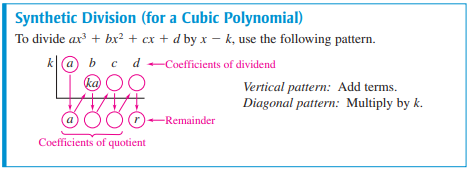
\includegraphics[width=4in]{SynDivBlock.png}
		
		\pause
		
		The setup is very similar for polynomials of degrees other than $3$.
	\end{frame}

	\begin{frame}{Synthetic Division of Polynomials}
		Divide $x^4 - 10x^2 - 2x + 4$ by $x + 3$ using synthetic division.
		
		\only<2>{\polyhornerscheme[x=-3,stage=1]{x^4 - 10x^2 - 2x + 4}}
		\only<3>{\polyhornerscheme[x=-3,stage=2]{x^4 - 10x^2 - 2x + 4}}
		\only<4>{\polyhornerscheme[x=-3,stage=3]{x^4 - 10x^2 - 2x + 4}}
		\only<5>{\polyhornerscheme[x=-3,stage=4]{x^4 - 10x^2 - 2x + 4}}
		\only<6>{\polyhornerscheme[x=-3,stage=5]{x^4 - 10x^2 - 2x + 4}}
		\only<7>{\polyhornerscheme[x=-3,stage=6]{x^4 - 10x^2 - 2x + 4}}
		\only<8>{\polyhornerscheme[x=-3,stage=7]{x^4 - 10x^2 - 2x + 4}}
		\only<9>{\polyhornerscheme[x=-3,stage=8]{x^4 - 10x^2 - 2x + 4}}
		\only<10>{\polyhornerscheme[x=-3,stage=9]{x^4 - 10x^2 - 2x + 4}}
		\only<11->{\polyhornerscheme[x=-3,stage=10]{x^4 - 10x^2 - 2x + 4}}
		
		\only<12>{This tells us that $(x^4 - 10x^2 - 2x + 4) \div (x + 3) = x^3 - 3x^2 - x + 1 + \dfrac{1}{x+3}$.}
	\end{frame}

	\begin{frame}{Synthetic Division of Polynomials}
		Divide $5x^3 + 8x^2 - x + 6$ by $x+2$ using synthetic division.
		
		\only<2>{\polyhornerscheme[x=-2, stage=1]{5x^3 + 8x^2 - x + 6}}
		\only<3>{\polyhornerscheme[x=-2, stage=2]{5x^3 + 8x^2 - x + 6}}
		\only<4>{\polyhornerscheme[x=-2, stage=3]{5x^3 + 8x^2 - x + 6}}
		\only<5>{\polyhornerscheme[x=-2, stage=4]{5x^3 + 8x^2 - x + 6}}
		\only<6>{\polyhornerscheme[x=-2, stage=5]{5x^3 + 8x^2 - x + 6}}
		\only<7>{\polyhornerscheme[x=-2, stage=6]{5x^3 + 8x^2 - x + 6}}
		\only<8>{\polyhornerscheme[x=-2, stage=7]{5x^3 + 8x^2 - x + 6}}
		\only<9>{\polyhornerscheme[x=-2, stage=8]{5x^3 + 8x^2 - x + 6}}
	\end{frame}

	\begin{frame}{The Remainder Theorem}
	We can use polynomial division to evaluate functions using the Remainder Theorem:
	\begin{block}{The Remainder Theorem}
		If a polynomial $f(x)$ is divided by $x - k$, then the remainder is $r = f(k)$.
	\end{block}

	\pause

	Example: Suppose that $f(x) = 4x^3 + 10x^2 - 3x - 8$. Evaluate $f(4)$ and $f(-3)$ using the Remainder Theorem. 
	
	\pause
	
	\polyhornerscheme[x = 4]{4x^3 + 10x^2 - 3x - 8} \pause \polyhornerscheme[x=-3]{4x^3 + 10x^2 - 3x - 8}
	
	\pause
	
	The Remainder Theorem tells us that $f(4)=396$ and $f(-3) = -17$ (confirm this).
	\end{frame}

	\begin{frame}{The Factor Theorem}
		\begin{block}{The Factor Theorem}
			A polynomial has a factor $(x-k)$ if and only if $f(k) = 0$
		\end{block}
	
		\pause Note that $f(k) = 0$ if and only if the remainder when $f(x)$ is divided by $x - k$ is $0$ (Remainder Theorem).
		
		\pause
		
		Example: Show that $2x-3$ is a factor of $f(x) = 10x^3 - x^2 - 37x + 24$ using the Factor Theorem.
		
		\pause
		
		Since the divisor isn't of the form $x - k$, we need to use long division.
	\end{frame}

	\begin{frame}{The Factor Theorem}
		\polylongdiv{10x^3 - x^2 - 37x  + 24}{2x-3}
		
		\pause
		
		Since the remainder is $0$, we can conclude that $2x - 3$ is a factor of $f(x) = 10x^3 - x^2 - 37x + 24$
	\end{frame}

	\begin{frame}{Next Steps}
	\begin{itemize}
		\item Post questions in Lesson 12 Forum, if you have any
		\item Read 3.4
		\item Watch Video Lesson \#13
		\item Complete Assignment \#6
	\end{itemize}

	\vfill
	
	Thanks for watching!
	\end{frame}
\end{document}